\documentclass[aspectratio=169,xcolor=dvipsnames]{beamer}
\usetheme{SimplePlus}

% Math
\usepackage{nicefrac}

% Tipography stuff
\usepackage{booktabs} % Allows the use of \toprule, \midrule and \bottomrule in tables
\usepackage[english]{babel}
\usepackage{microtype}
\usepackage{pdfpages}
\usepackage{fontawesome5}
\usepackage{soul}
\usepackage{euler}
\usepackage{algorithm2e}

% Bibliography
\usepackage[giveninits,style=authoryear-comp,backend=biber]{biblatex}
\addbibresource{../fracbiblio.bib}
\newcommand\unnumbered{\setbeamertemplate{footline}{}}%\addtocounter{framenumber}{-1}
\renewcommand*{\bibfont}{\normalfont\small}

% Figures
\usepackage{tikz,pgfplots}
\usetikzlibrary{calc,arrows,patterns}
\usepackage{subfig}
\usepackage{graphicx} % Allows including images
\usepackage[american]{circuitikz}

% Links
\usepackage{hyperref}
\hypersetup{colorlinks,linkcolor=,urlcolor=MidnightBlue}

% Code
\usepackage{minted}

% Block matrices
\newcommand{\bigzero}{\mbox{\normalfont\Large\bfseries 0}}
\newcommand{\rvline}{\hspace*{-\arraycolsep}\vline\hspace*{-\arraycolsep}}


\author{Fabio Durastante}
\title{An introduction to fractional calculus}
\subtitle{Fundamental ideas and numerics}
\institute{Università di Pisa\\\href{mailto:fabio.durastante@unipi.it}{\faEnvelope\;fabio.durastante@unipi.it}\\\href{https://fdurastante.github.io}{\faFirefox\;fdurastante.github.io}}
\date{June, 2022}

\newcommand{\de}{{\rm d}}


\begin{document}

{\unnumbered
\begin{frame}[t,plain,noframenumbering]
\titlepage
\vspace{-4em}
\includegraphics[width=2cm]{frame.png}
\end{frame}
}

\section{Subdiffusion equations}

\begin{frame}{Subdiffusion equations}
At the end of the last lecture we had observed the following behavior:

\begin{center}
	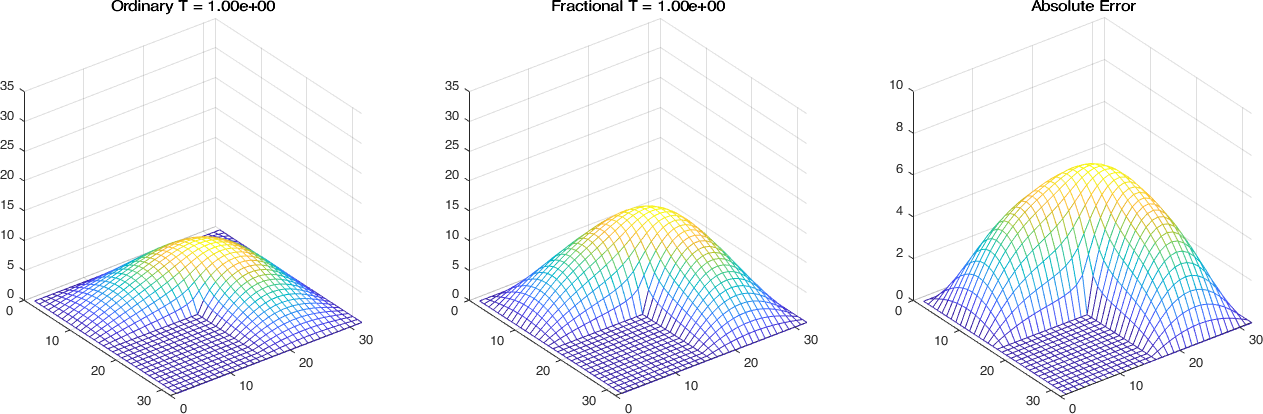
\includegraphics[width=0.8\columnwidth]{diff_101.png}
\end{center}

for the solution of:
\[
{}_{CA}D^{\alpha}_t u = 0.05 \nabla^2 u, \quad \alpha = 0.3,1.
\]
The \alert{visual effect} seemed to be a \textbf{slowing down of the diffusion}.
\end{frame}

\begin{frame}{Brownian motion~\parencite{MR1809268}}
\begin{itemize}
\item Consider a 1D lattice with cell size $\Delta x$,
\item In discrete time steps of span $\Delta t$ a test particle jumps to one of its neighbour sites,
\item<2-> The process can be modelled by the master equation
\[
W_{j}(t+\Delta t) = \frac{1}{2} W_{j-1}(t) + \frac{1}{2}W_{j+1}(t)
\]
\only<10->{
\item<11-> The master equation defines the \emph{pdf} to be at position $j$ at time $t + \Delta t$ depending on the population of the two adjacent sites $j\pm 1$ at time $t$.
\item<12-> The prefactor $\nicefrac{1}{2}$ tells us that the \textbf{process is isotropic} with respect to the left/right direction.
\item<13-> If we let $\Delta t \rightarrow 0$, $\Delta x \rightarrow 0$ and do a \alert{Taylor expansion} in both $\Delta$ and $\Delta x$ we get
\[
\begin{split}
W_j(t+\Delta t) = & W_j(t) + \Delta t \frac{\partial W_j}{\partial t} + O([\Delta t]^2), \qquad \text{ for } \Delta t \rightarrow 0,\\
W_{j\pm1}(t) = & W(x,t) \pm \Delta x \frac{\partial W}{\partial x} + \frac{(\Delta x)^2}{2} \frac{\partial^2 W}{\partial x^2} + O([\Delta x]^3) , \qquad \text{ for } \Delta x \rightarrow 0,
\end{split}
\]	
}
\end{itemize}

\only<1-9>{\begin{center}
\only<2>{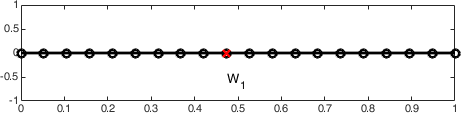
\includegraphics[width=0.8\columnwidth]{randomwalk1_01.png}}%\
\only<3>{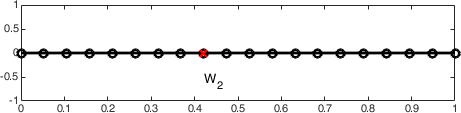
\includegraphics[width=0.8\columnwidth]{randomwalk1_02.png}}%\
\only<4>{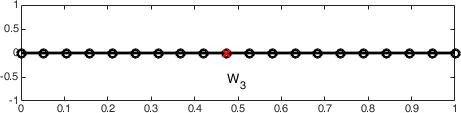
\includegraphics[width=0.8\columnwidth]{randomwalk1_03.png}}%\
\only<5>{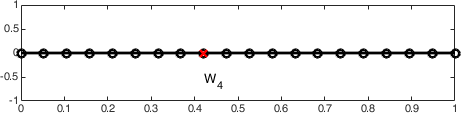
\includegraphics[width=0.8\columnwidth]{randomwalk1_04.png}}%\
\only<6>{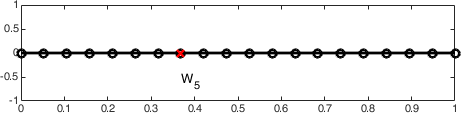
\includegraphics[width=0.8\columnwidth]{randomwalk1_05.png}}%\
\only<7>{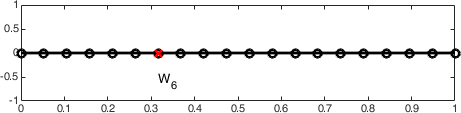
\includegraphics[width=0.8\columnwidth]{randomwalk1_06.png}}%\
\only<8>{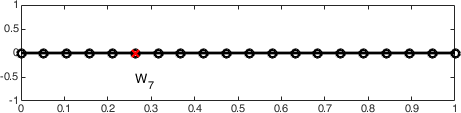
\includegraphics[width=0.8\columnwidth]{randomwalk1_07.png}}%\
\only<9>{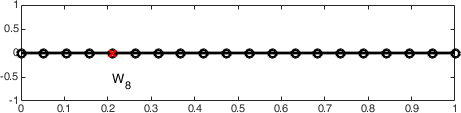
\includegraphics[width=0.8\columnwidth]{randomwalk1_08.png}}%\
\end{center}}

\end{frame}

\begin{frame}{Brownian motion~\parencite{MR1809268}}
We now substitute the expansions
\[
\begin{split}
W_j(t+\Delta t) = & W_j(t) + \Delta t \frac{\partial W_j}{\partial t} + O([\Delta t]^2), \qquad \text{ for } \Delta t \rightarrow 0,\\
W_{j\pm1}(t) = & W(x,t) \pm \Delta x \frac{\partial W}{\partial x} + \frac{(\Delta x)^2}{2} \frac{\partial^2 W}{\partial x^2} + O([\Delta x]^3) , \qquad \text{ for } \Delta x \rightarrow 0,
\end{split}
\]	
in
\[
W_{j}(t+\Delta t) = \frac{1}{2} W_{j-1}(t) + \frac{1}{2}W_{j+1}(t)
\]
obtaining
\only<1>{
\[
W(x,t)+\text{$\Delta $t} \frac{\partial W}{\partial t}+O\left(\text{$\Delta $t}^2\right)=W(x,t)+\frac{1}{2} \text{$\Delta $x}^2 \frac{\partial^2 W}{\partial x^2}+O\left(\text{$\Delta $x}^3\right)
\]}\only<2>{
\[
\frac{\partial W}{\partial t} = \frac{\Delta x^2}{2\Delta t} \frac{\partial^2 W}{\partial x^2} + O\left(\text{$\Delta $x}^3 + \Delta t \right)
\]}\only<3>{
\[
\frac{\partial W}{\partial t} = K_1 \frac{\partial^2 W}{\partial x^2}, \qquad K_1 = \lim_{\substack{\Delta x \rightarrow 0\\\Delta t \rightarrow 0}} \frac{\Delta x^2}{2\Delta t} < \infty.
\]
}
\end{frame}

\begin{frame}{Brownian motion}
\[
\frac{\partial W}{\partial t} = K_1 \frac{\partial^2 W}{\partial x^2}
\]
Let us call $X$ the random variable measuring the distance covered in two consecutive jumps
\begin{itemize}
	\item Assume that the \emph{pdf} of $X$ (appropriately normalised) has existing moments
	\[
	\overline{X} = \sum_{i} X_i, \qquad \overline{X^2},
	\]
	and mean time-span $\Delta t$ between any two individual jump events.
	\item<2-> Then the \textbf{central limit theorem} assures that exists
	\[
	V = \frac{\overline{X}}{\Delta t}\;\text{(Mean velocity)}\quad K = \frac{\overline{X^2}-\overline{X}^2}{2\Delta t}\;\text{(Diffusion coefficient)}
	\]
	and that
	\[
	W(x,t) = \frac{1}{2\sqrt{\pi K_1 t}} \exp\left(- \nicefrac{x^2}{4K_1 t}\right).
	\]
\end{itemize}
\end{frame}

\begin{frame}{Brownian motion: the Fourier domain}

We can rewrite
\[
W(x,t) = \frac{1}{2\sqrt{\pi K_1 t}} \exp\left(- \nicefrac{x^2}{4K_1 t}\right).
\]
in the \textbf{Fourier domain} as
\[
W(k,t) = \exp(-K_1 k^2 t), \qquad W_0(x) = \lim_{t\rightarrow0^+} W(x,t) = \delta(x),
\]
that solve the \alert{Fourier transformed diffusion equation}
\[
\frac{\partial W}{\partial t} = - K_1 k^2 W(k,t),
\]
that is a \textbf{relaxation equation}, for a fixed wavenumber $k$.
\end{frame}

\begin{frame}{From the discrete to the continuous}

The \alert{\textbf{C}}ontinuous \alert{\textbf{T}}ime \alert{\textbf{R}}andom \alert{\textbf{W}}alk model (CTRW):
\begin{itemize}
	\item[\faLightbulb] Both the \textbf{length of a given jump}, and the \textbf{waiting time}
	elapsing between two successive jumps are drawn from a pdf $\psi(x,t)$
	\item[\faWalking]<2-> The jump length pdf
	\[
	\lambda(x) = \int_{0}^{+\infty} \psi(x,y)\,\textrm{d}t,
	\]
	\begin{onlyenv}<2>
	\begin{exampleblock}{Jump length}
	$\lambda(x) \textrm{d}x$ produces the probability for a jump length in the interval $(x,x+\textrm{d}x)$.
	\end{exampleblock}
	\end{onlyenv}
	\item[\faClock]<3-> The waiting time pdf
	\[
	w(t) = \int_{-\infty}^{+\infty} \psi(x,t)\,\textrm{d}x
	\]
	\begin{onlyenv}<3>
	\begin{exampleblock}{Waiting time}
		$w(t) \textrm{d}t$ produces the probability for a waiting time in the interval $(t,t+\textrm{d}t)$.
	\end{exampleblock}
	\end{onlyenv}
	\only<4->{
	\item If the jump length and
	waiting time are \textbf{independent random variables} then: \[\psi(x,t) = w(t)\lambda(x)\]
	}
\end{itemize}

\end{frame}

\begin{frame}{Characterization of CTRW}
To categorise different CTRW one can look at the quantities
\[
T = \int_{0}^{+\infty} t w(t)\,\textrm{d}t, \text{ (Characteristic waiting time)},
\]
and 
\[
\Sigma^2 = \int_{-\infty}^{+\infty} x^2\lambda(x)\,\textrm{d}x\, \text{ (Jump length variance)},
\]
specifically, are they \textbf{finite}? Do they \textbf{diverge}?

\onslide<2->{
The \alert{master} (Langevin) \alert{equation} for this process is then given by
\[
\alert<3>{\eta(x,t)} = \int_{-\infty}^{+\infty} \textrm{d}x' \int_{0}^{+\infty} \textrm{d}t'\,\alert<4>{\eta(x',t')} \psi(x-x',t-t') + \delta(x)\delta(t),
\]
\only<3->{Pdf of having arrived at position $x$ at time $t$ -- $\eta(x,t)$ --}\only<4->{ having just arrived at $x'$ at time $t'$ -- $\eta(x',t')$ --}\only<5->{ with initial condition $\delta(x)$.}
}

\end{frame}

\begin{frame}{Characterization of CTRW}
Then if we use 
\[
\eta(x,t) = \int_{-\infty}^{+\infty} \textrm{d}x' \int_{0}^{+\infty} \textrm{d}t'\,\eta(x',t') \psi(x-x',t-t') + \delta(x)\delta(t),
\]
we can write the pdf of being in $x$ at time $t$ as
\[
W(x,t) = \int_{0}^{t} \eta(x,t') \Psi(t-t'),\textrm{d}t, \qquad \Psi(t) = 1 - \int_{0}^{t} w(t')\,\textrm{d}t',
\]
where the latter is the cumulative probability assigned to the probability of \alert{no jump event} during the time interval  $t-t'$.
\begin{alertblock}{Fact}
If both $T$ and $\Sigma^2$ are finite the long-time limit corresponds to Brownian motion, e.g., $w(t) = \tau^{-1} exp(-\nicefrac{t}{\tau})$, $T = \tau$, $\lambda(x) = (4\pi \sigma^2)^{-\nicefrac{1}{2}} \exp(-\nicefrac{x^2}{4\sigma^2})$, $\Sigma^2 = 2 \sigma^2$, we recover the standard diffusion equation.
\end{alertblock}
\end{frame}

\begin{frame}{The CTRW in the Fourier-Laplace domain}

We take
\[
W(x,t) = \int_{0}^{t} \eta(x,t') \Psi(t-t'),\textrm{d}t, \qquad \Psi(t) = 1 - \int_{0}^{t} w(t')\,\textrm{d}t',
\]
and rewrite it again in the \textbf{Fourier-Laplace domain} (Fourier for the space variable, Laplace for the time one) as
\[
W(k,u) = \frac{1-w(u)}{u} \frac{W_0(k)}{1-\psi(k,u)}, \qquad W_0(k) = \int_{-\infty}^{+\infty} W_0(x) e^{-i 2 \pi k x}\,\textrm{d}x.
\]
In the \textbf{Brownian case}
\[
w(u) \sim 1 - u\tau + O(\tau^2), \quad \lambda(k) \sim 1 - \sigma^2 k^2 + O(k^4), \quad W_0(x) = \delta(x)
\]
then
\[
W(k,u) = \frac{1}{u + K_1 k^2}, \quad K_1 = \nicefrac{\sigma^2}{\tau}.
\]

\end{frame}

\begin{frame}{The case of long rests}

\begin{block}{\faBed\; Long rests}
The \textbf{characteristic waiting time} $T = \int_{0}^{+\infty} t w(t)\,\textrm{d}t$ \textbf{diverges}, but the jump length variance $\Sigma^2 = \int_{-\infty}^{+\infty} x^2\lambda(x)\,\textrm{d}x$ is finite.
\end{block}

\begin{itemize}
	\item<2-> To realize this we can select
	\[
	w(t) \sim  A_\alpha \left(\nicefrac{\tau}{t}\right)^{1+\alpha}, \qquad 0 < \alpha < 1,
	\]
	\item<3-> For the jump pdf we use again the Gaussian jump length
	\[
	\lambda(x) = (4\pi \sigma^2)^{-\nicefrac{1}{2}} \exp(-\nicefrac{x^2}{4\sigma^2}).
	\]
	\item<4-> To get the form of the equation we first go to the Laplace domain:
	\[
	w(u) \sim 1 - (u\tau)^\alpha,
	\]
	\item<5-> and then obtain the expression for $W(k,u)$ in the Fourier-Laplace space
	\[
	W(k,u) = \nicefrac{\nicefrac{W_0(k)}{u}}{\left(1 + K_\alpha u^{-\alpha} k^2\right)}.
	\]
\end{itemize}

\end{frame}

\begin{frame}{The case of long rests}

To get an expression of the equation we use the Laplace transform for fractional integrals:
\[
\mathcal{L}\left\lbrace I_{[0,t]}^{-\alpha} W(x,t) \right\rbrace = u^{-\alpha} W(x,u), \qquad \alpha \geq 0,
\]
and together with 
\[
W(k,u) = \frac{\nicefrac{W_0(k)}{u}}{\left(1 + K_\alpha u^{-\alpha} k^2\right)}.
\]
we infer the fractional integral equation\only<2>{, and apply derivative w.r.t. to time}
\only<1>{\[
W(x,t) - W_0(x) = I_{[0,t]} K_{\alpha} \frac{\partial^2}{\partial x^2} W(x,t).
\]}%
\only<2>{\[
\frac{\partial}{\partial t} \left( W(x,t) - W_0(x) \right) = \frac{\partial}{\partial t} \left( I_{[0,t]} K_{\alpha} \frac{\partial^2}{\partial x^2} W(x,t) \right).
\]
}%
\only<3->{
\[
\frac{\partial W}{\partial t} = {}_{RL}D_{[0,t]}^\alpha K_\alpha \frac{\partial^2}{\partial x^2} W(x,t).
\]	
}%
\only<4>{
We can compute also the mean squared displacement
\[
\langle x^2(t) \rangle = \mathcal{L}^{-1} \left\lbrace \lim_{k \rightarrow 0} - \frac{d^2}{dk^2}W(k,u) \right\rbrace = \frac{2 K_\alpha}{\Gamma(1+\alpha)}t^\alpha. 
\]
}
\end{frame}

\begin{frame}{The case of long rests}
We have obtained a Fractional Differential Equation:
\[
\frac{\partial W}{\partial t} = {}_{RL}D_{[0,t]}^\alpha K_\alpha \frac{\partial^2}{\partial x^2} W(x,t), \qquad 0 < \alpha < 1
\]
but this is not the model we started looking at, that was
\[
{}_{CA}D_{[0,t]}^\alpha W = K_\alpha \frac{\partial^2}{\partial x^2} W(x,t), \qquad 0 < \alpha < 1
\]
\faQuestionCircle\;\alert{Are they related?} \onslide<2->{It turns out that this is indeed the case~\parencite{MR2150232}, the proof involves doing some work in inverting Fourier-Laplace transform.}\vfill

\onslide<3>{We now have an \emph{interpretation} of what a Fractional Derivative with respect to time is. We will come back to this when we will speak about fractional derivative with respect to space.}

\end{frame}

\section{``Exponential'' Fractional Integrators}

\begin{frame}{``Exponential'' Fractional Integrators}

We start from the FDE
\[
\begin{cases}
{}_{CA}D^\alpha_{[t_0,t]} u(t) + \lambda y(t) = f(t), \\
u(0) = u_0,
\end{cases} \; \alpha \in \mathbb{R}_{> 0}, \quad \lambda \in \mathbb{R}, \; u(t)\,:[t_0,T] \rightarrow \mathbb{R}.
\]
Then we rewrite the solution as
\[
u(t) = e_{\alpha,1}(t-t_0;\lambda) u_0 + \int_{t_0}^{t} e_{\alpha,\alpha}(t-s;\lambda) f(s)\,\textrm{d}s, \quad e_{\alpha,\beta} = t^{\beta - 1} E_{\alpha,\beta}(-\lambda t^\alpha),
\]
for $E_{\alpha,\beta}(z)$ the Mittag-Leffler (ML) function with two parameters.

\begin{itemize}
	\item[\faLightbulb]<2-> We can use this formulation to build different PI rules,
	\item[\faLightbulb]<3-> We can use it to address the problem
	\[
	{}_{CA}D^\alpha_{[t_0,t]} U(t) + A y(t) = F(U(t)), \quad U(0) = U_0.
	\]
\end{itemize}

\end{frame}

\begin{frame}{Evaluation of the ML function}
For both the approaches we need reliable ways for \textbf{computing} the \textbf{ML function} on both the \textbf{real line} and with \textbf{matrix argument}.  
\begin{description}
	\item[Scalar case]<2-> Inversion of the Laplace transform via the \alert{Optimal Parabola Contour} selection algorithm~\parencite{Garrappa},
	\item[Matrix argument]<3-> To apply algorithm for matrix-function evaluation we may need also the value of the derivative of the ML function, e.g., Schur-Parlett type algorithm~\parencite{MatrixML,HighamML}. 
\end{description}

\onslide<3->{In general, we expect to mostly need matrix function--times--vector operations:
\[
\mathbf{y} = E_{\alpha,\beta}(A) \mathbf{v}, \qquad A \in \mathbb{R}^{n \times n}, \quad \mathbf{y},\mathbf{v} \in \mathbb{R}^n.
\]
}\vfill

\onslide<4>{We postpone it to after we have discussed the actual necessities we have.}

\end{frame}

\begin{frame}{PI - ``Exponential'' Fractional Integrators}
We start from the formula
\[
u(t) = e_{\alpha,1}(t-t_0;\lambda) u_0 + \int_{t_0}^{t} e_{\alpha,\alpha}(t-s;\lambda) f(s)\,\textrm{d}s, \quad e_{\alpha,\beta} = t^{\beta - 1} E_{\alpha,\beta}(-\lambda t^\alpha),
\]
and select a grid $\{t_i\}_{i=0}^{N}$, then
\only<1-3>{\[
u(t_n) = e_{\alpha,1}(t_n - t_0;\lambda) u_0 + \sum_{j=0}^{n-1} \alert<3>{\int_{t_j}^{t_{j+1}} e_{\alpha,\alpha}(t_n - s;\lambda) f(s)\,\textrm{d}s}.
\]}
\only<4->{\[
	u(t_n) = e_{\alpha,1}(t_n - t_0;\lambda) u_0 + \tau^\alpha \sum_{j=0}^{n-1} \int_{0}^{1} e_{\alpha,\alpha}(\nicefrac{(t-t_j)}{\tau} - r;\tau^\alpha \lambda) f(t_j + r\tau)\,\textrm{d}r.
\]}
\begin{itemize}
	\item<2-> In general we have \[e_{\alpha,\beta}(t;\lambda) = \tau^{\beta-1} e_{\alpha,\beta}(\nicefrac{t}{\tau};\tau^\alpha \lambda)\]
	\item<3-> For $s \in [t_j,t_{j+1}]$ let us consider the \emph{change of variables} $s = t_j + r\tau$, $r \in [0,1]$ 
\end{itemize}
\end{frame}

\begin{frame}{PI - ``Exponential'' Fractional Integrators}
\only<1>{Then a PI rule for
\[
u(t_n) = e_{\alpha,1}(t_n - t_0;\lambda) u_0 + \tau^\alpha \sum_{j=0}^{n-1} \int_{0}^{1} e_{\alpha,\alpha}(\nicefrac{(t-t_j)}{\tau} - r;\tau^\alpha \lambda) \alert<1>{f(t_j + r\tau)}\,\textrm{d}r.
\]}%
\only<2>{Then the PI rule is
\[
u^{(n)} = e_{\alpha,1}(t_n - t_0;\lambda)y_0 + \tau^\alpha \sum_{j=0}^{n-1} \sum_{\ell = 0}^{q} \omega_\ell^{[q;\alpha]}(n-j;\tau^\alpha \lambda) f(t_j + c_\ell\tau).
\]
}
is obtained by selecting $q+1$ \emph{distinct} nodes $0 \leq c_0 < c_1 < \cdots < c_q \leq 1$ and replacing $f(t_j + r\tau)$ with
\[
p_j^{[q]}(t_j + r \tau) = \sum_{\ell=0}^{q} L_\ell^{[q]}(r) f(t_j + c_\ell \tau), \quad r \in [0,1], \quad L_\ell^{[q]} \text{ Lagrange basis element of degree }q.
\]
\onslide<2>{
And selecting the weights
\[
\omega_\ell^{[q;\alpha]}(n,z) = \int_{0}^{1}e_{\alpha,\alpha}(n-j-r;z) L_\ell^{[q]}(r)\,\textrm{d}r.
\]
}
\end{frame}

\begin{frame}{PI - ``Exponential'' Fractional Integrators}

\begin{alertblock}{Theorem \parencite[Theorem 4.2]{GarrappaPopolizioPIExponential}}
Let $\alpha > 0$ and $f(t) \in \mathcal{C}^{q+2}([t_0,T])$. The error of a $q$-step exponential PI rule is given by
\[
u(t_n) - u^{(n)} = \tau^{q+1} \frac{C_0^{[q]}}{(q+1)!} \int_{t_0}^{t_n} e_{\alpha,\alpha}(t_n-s;\lambda) f^{(q+1)}(s)\,\textrm{d}s + O(\tau^{q+1+\alpha}),
\]
where the constant $C_0^{[q]}$ depends only on the nodes $c_\ell$.
\end{alertblock}

\begin{itemize}
	\item For $q = 2$, $c_0 = 0$, $c_1 = \nicefrac{1}{2}$ $c_2 = 1$, one finds $C^{[2]}_0 = 0$, thus an interpolatory formula of order $O(\tau^{q+1+\alpha})$. 
	\item[\faLightbulb] The \textbf{general idea} is to select nodes $c_\ell$ in such way that 
	\[
	C_\nu^{[q]} = \int_{0}^{1} \omega_q(r) \xi(1-\nu,1-r)\,\textrm{d}r, \quad \nu \in \mathbb{R},
	\]
	for $\xi$ the \emph{Hurwitz zeta function}, are zeroed out in the error expansion for the method.
\end{itemize}

\end{frame}

\section{The MOL/Matrix case}

\begin{frame}{The MOL/Matrix case}
Let us go back to the case that sparked our interest in going ``exponential'', that was the MOL problem
\[
\begin{cases}
{}_{CA}D^\alpha_{[0,t]} \mathbf{u}(t) + A\mathbf{u}(t) = \mathbf{g}(t), & t > 0,\\
\mathbf{u}(0) = \mathbf{u}_0.
\end{cases}
\]
By the variation of constant formula, we have seen that we can express the solution as
\[
\mathbf{u}(t) = E_{\alpha,1}(-t^\alpha A) \mathbf{u}_0 + \int_{0}^{t} (t-s)^{\alpha-1} E_{\alpha,\alpha}(-A(t-s)^\alpha)\mathbf{g}(s)\,\textrm{d}s.
\]
\begin{itemize}
	\item<2-> In the general case we then have to apply one of the PI rules to compute the integral term, 
	\item<3-> If $g(s) = \sum_{k=0}^q s^k \mathbf{v}_k$ for some vectors, we can compute the integral on the right-hand side in \emph{closed form} and obtain
	\[
	\mathbf{u}(t) = E_{\alpha,1}(-t^\alpha A)\mathbf{y}_0 + \sum_{k=0}^{q} \Gamma(k+1) t^{\alpha+k} E_{\alpha,\alpha+k+1}(-t^\alpha A)\mathbf{v}_k, \qquad t > 0.
	\]
\end{itemize}

\end{frame}

\begin{frame}{Matrix functions: the normal case}

If $A$ is a normal matrix, and $f$ is a function existing on the spectrum of $A$, then
\[
f(A) = U f(\Lambda) U^H, \quad U^HU= I, \quad \Lambda = \operatorname{diag}(\lambda_1,\ldots,\lambda_n),\; A \mathbf{u}_i = \lambda_i \mathbf{u}_i, \quad U = [\mathbf{u}_1,\ldots,\mathbf{u}_n].
\]
This is, e.g., sufficient for the cases in which
\begin{itemize}
	\item $A$ is the discretization of a self-adjoint operator,
	\item $A$ is symmetric.
\end{itemize}
$E_{\alpha,\beta}(z)$ is an \textbf{analytic function}, and therefore we can compute it for every possible eigenvalue $\lambda$ in the spectrum of $A$.\vfill

\onslide<2>{What about the \emph{non-normal} and \emph{nond-diagonalizable} case? For diagonalizable matrices, we can use the eigendecomposition at the same way.}

\end{frame}

\begin{frame}{Matrix functions: the Jordan Canonical Form}

\begin{block}{Jordan Canonical Form}
We recall that any matrix $A \in \mathbb{C}^{n \times n}$ can be expressed in Jordan canonical
form as
\begin{equation*}
Z^{-1} A Z = J = \operatorname{diag}(J_1,\ldots,J_p), \quad \text{ for }
J_k = J_k(\lambda_k) = \begin{bmatrix}
\lambda_k & 1 \\
& \lambda_k & \ddots \\
& & \ddots & 1 \\
& & & \lambda_k
\end{bmatrix} \in \mathbb{C}^{m_k \times m_k},
\end{equation*}
where $Z$ is nonsingular and $m_1 + m_2 + \ldots + m_p = n$. If each block in which the eigenvalue $\lambda_k$ appears is of size 1 then $\lambda_k$ is said to be a \textit{semisimple} eigenvalue.
\end{block}
\begin{itemize}
	\item This is a \emph{theoretical object}, it is useful to prove and define \emph{things}, \alert{not to implement \emph{things}}.
	\item<2-> Now that we have a decomposition of the matrix, we need to introduce a suitable definition of \textbf{being defined on the spectrum}.
\end{itemize}

\end{frame}

\begin{frame}{Matrix functions: the general case}

Let us denote by $\lambda_1,\ldots,\lambda_s$ the distinct
eigenvalues of $A$, and by $n_i$ the order of the largest Jordan block in
which the $\lambda_i$ appears, i.e., the \textit{index} of the eigenvalue
$\lambda_i$.

\begin{block}{Defined on the spectrum}
The function $f$ is \textit{defined on the spectrum of} $A$ if the values
\begin{equation*}
f^{(j)}(\lambda_i), \qquad j=0,1,\ldots,n_i-1, \quad i = 1,\ldots s,
\end{equation*}
exist, where $f^{(j)}$ denotes the $j$th derivative of $f$, with $f^{(0)} = f$.
\end{block}

\begin{itemize}
	\item[\faExclamationTriangle]<2-> Again for the ML function and $\alpha > 0$ we have no problem with this. 
\end{itemize}

\end{frame}

\begin{frame}{Matrix functions: the general case}
\begin{block}{Matrix function}
	Lef $f$ be defined on the spectrum of $A \in \mathbb{C}^{n \times
		n}$, which is represented in Jordan canonical form as $Z^{-1}AZ = J$,\vspace{-0.5em}
	\begin{equation*}
	f(A) = Z f(J) Z^{-1} = Z \operatorname{diag}(f(J_1),\ldots,f(J_p))Z^{-1},
	\end{equation*}
	where\vspace{-0.5em}
	\begin{equation*}
	f(J_k) = \begin{bmatrix}
	f(\lambda_k) & f'(\lambda_k) & \ldots & \frac{f^{(m_k-1)}(\lambda_k)}{(m_k-1)!} \\
	& f(\lambda_k) & \ddots & \vdots \\
	& & \ddots & f'(\lambda_k) \\
	& & & f(\lambda_k)
	\end{bmatrix}.
	\end{equation*}
	Moreover, let $f$ be a multivalued function and suppose some eigenvalues occur in more than one Jordan block. If the same choice of branch of $f$ is made in each block, then we say that $f(A)$ is a \textit{primary matrix function}.
\end{block}
\end{frame}

\begin{frame}{Matrix functions: computing $f(A)$ and $f(A)\mathbf{v}$}
To march our scheme for
\[
\mathbf{u}(t) = E_{\alpha,1}(-t^\alpha A) \mathbf{u}_0 + \int_{0}^{t} (t-s)^{\alpha-1} E_{\alpha,\alpha}(-A(t-s)^\alpha)\mathbf{g}(s)\,\textrm{d}s.
\]
we need to compute operations of the form $f(A)\mathbf{v}$, \emph{nevertheless}, we will have to compute $f(\cdot)$ at least on some \alert{small matrix}.

\begin{block}<2->{Schur decomposition and matrix functions}
Given a matrix $A$ there exist always a matrix $Q$ such that $Q^*Q = I$, and a upper triangular matrix $T$ such that $A = Q T Q^*$. Then, if $f$ is \alert{defined on the spectrum} of $A$ we can compute $f(A)$ as $f(A) = Q f(T) Q^*$.
\end{block}

\begin{onslide}<3>
But how do we compute the matrix function of an upper triangular matrix?
\end{onslide}

\end{frame}

\subsection{The case of small matrices}

\begin{frame}{Matrix functions: the upper triangular case}
\begin{description}
	\item[Assumption] we assume that $T$ is such that each block $T_{i,j}$ has \alert{clustered eigenvalues}, and distinct diagonal blocks have \emph{far enough} eigenvalues. 
	\item[\faExclamationCircle] If the \textbf{assumption} doesn't hold we look for a block permutation.
\end{description}
\begin{columns}
\begin{column}{0.5\columnwidth}
\[
\begin{bmatrix}
\begin{matrix}
\alert<2>{(T_{1,1})_{1,1}} & \alert<2>{(T_{1,1})_{1,2}} \\
\alert<2>{0} & \alert<2>{(T_{1,1})_{2,2}}
\end{matrix}
& \rvline & \mbox{\normalfont\Large \alert<3>{$T_{1,2}$} } \\
\hline
\bigzero & \rvline &
\begin{matrix}
\alert<2>{(T_{2,2})_{1,1}} & \alert<2>{(T_{2,2})_{1,2}} \\
\alert<2>{0} & \alert<2>{(T_{2,2})_{2,2}}
\end{matrix}
\end{bmatrix}
\]
\onslide<1>{\alert{\faExclamationTriangle} Close eigenvalues may lead to severe \emph{accuracy loss}, even far apert eigenvalues can produce more inaccurate answers than expected, see~\parencite{DaviesHighamSchurParlett}.}
\end{column}
\begin{column}{0.5\columnwidth}
\only<2>{
\begin{itemize}
	\item<2-> To evaluate $f(T_{ii})$ we use the Taylor series in $\sigma$
	\[
	f(T_{i,i}) = \sum_{k=0}^{+\infty} \frac{f^{(k)}}{k!} M^{k},
	\]
	for $\sigma = \nicefrac{\operatorname{trace}(T_{i,i})}{m}$, $m = \dim(T_{i,i})$, and $M = T_{i,i} - \sigma I$.
\end{itemize}}
\only<3>{For the \alert<3>{off-diagonal blocks} we apply the block-Parlett recurrence
\begin{algorithm}[H]
$F_{i,i} = f(T_{i,i})$, $i=1,\ldots,n$\;
\For{$j=2,\ldots,n$}{
\For{$i=j-1,j-2,\ldots,1$}{
	Solve Sylvester equation for $F_{i,j}$:\\ 
	$T_{i,i} F_{j,j} - F_{i,j} T_{j,j} = F_{i,i} T_{i,j} - T_{i,j} F_{j,j}$\\ $+ \sum_{k=0}^{j-1}(F_{i,k}-T_{k,j} - T_{i,k}F_{k,j})$.
}
}
\end{algorithm}
}
\only<4>{
\begin{exampleblock}{What we need}
To use the algorithm we have sketched out, we need to be able to compute the derivatives of the ML function sufficiently accurately.
\end{exampleblock}
}
\end{column}
\end{columns}
\end{frame}

\begin{frame}{Derivatives of the ML function}
The key observation for this task is
\[
\frac{d^k}{d z^k} E_{\alpha,\beta}(z) = \sum_{j=0}^{+\infty} \frac{(j+k)_k z^j}{\Gamma(\alpha j + \alpha k + \beta)} = \frac{k!}{\Gamma(k+1)}\sum_{j=0}^{+\infty} \frac{\Gamma(j+k+1) z^j}{j!\Gamma(\alpha j + \alpha k + \beta)} = k! E_{\alpha,\alpha k + \beta}^{k+1} (z),
\]
where
\[
E_{\alpha,\beta}^\gamma(z) = \frac{1}{\Gamma(\gamma)} \sum_{j=0}^{+\infty} \frac{\Gamma(1+\gamma)z^j}{j! \Gamma(\alpha j + \beta)},
\]
is called the \alert{Prabhakar function}.

\onslide<2>{
Its \textbf{efficient computation} can be obtained, similarly to the ML function, by means of a \emph{Laplace transform inversion}
\[
\mathcal{L} \left\lbrace t^{\beta-1} E_{\alpha,\beta}^\gamma(t^\alpha z) \right\rbrace(s) = \frac{s^{\alpha\gamma-\beta}}{(s^\alpha-t^\alpha z)^\gamma}, \quad \Re(s) > 0, \quad |t^\alpha zs^{-\alpha}| < 1.
\]
}
\end{frame}

\begin{frame}[fragile]{Computing the Prabhakar function~\parencite{Garrappa}}

\only<1>{We select $t = 1$ in\[
\mathcal{L} \left\lbrace t^{\beta-1} E_{\alpha,\beta}^\gamma(t^\alpha z) \right\rbrace(s) = \frac{s^{\alpha\gamma-\beta}}{(s^\alpha-t^\alpha z)^\gamma}, \quad \Re(s) > 0, \quad |t^\alpha zs^{-\alpha}| < 1.
\]}\only<2->{Having selected $t=1$ we have
\[
\mathcal{L} \left\lbrace E_{\alpha,\beta}^\gamma(z) \right\rbrace(s) = \frac{s^{\alpha\gamma-\beta}}{(s^\alpha-z)^\gamma}, \quad \Re(s) > 0, \quad |zs^{-\alpha}| < 1\only<2>{.}\only<3->{,\; H_k(z;z) = \frac{s^{\alpha-\beta}}{(s^\alpha-z)^{k+1}}.}
\]
}
\begin{columns}
\begin{column}{0.7\columnwidth}
\begin{itemize}
	\item<3-> Since
	\[
	\frac{d^k}{d z^k} E_{\alpha,\beta}(z) = k! E_{\alpha,\alpha k + \beta}^{k+1} (z) = \frac{k!}{2\pi i} \int_{\mathcal{C}} e^s H_k(s;z)\textrm{d}s \equiv I_k(z),
	\]
	\item<4-> we use the \emph{Optimal Parabolic Contour} we have already discussed in \textbf{Lecture 2} to determine the deformation of the Bromwich line to evaluate
	\[
	I_{k}^{[N]} = \frac{k! h}{2\pi i}\sum_{j=-N}^{N} e^{\sigma(u_j)} H_k(\sigma(u_j);z) \sigma'(u_j).
	\] 
\end{itemize}
\end{column}
\begin{column}{0.3\columnwidth}
\only<4->{
\centering 
\begin{tikzpicture}
\begin{axis}[
width=\columnwidth,
height=\columnwidth,
axis x line=center,
axis y line=center,
xlabel={$\Re(z)$},
ylabel={$\Im(z)$},
xticklabels={,,},
yticklabels={,,},
xlabel style={below right},
ylabel style={above left},
xmin=-5,
xmax=5,
ymin=-5,
ymax=5]
\addplot[red,domain=-10:10] plot[smooth]({-0.25*x^2+2},{x});
\addplot[mark=*] coordinates {(2,0)} node[pin=-20:{$\sigma$}]{} ;
\addplot[mark=x,blue] coordinates {(1,1)};
\addplot[mark=x,blue] coordinates {(1,-1)};
\end{axis}
\end{tikzpicture}

$s = \mu (i u + 1)^2,\; - \infty < u < \infty$
}
\end{column}
\end{columns}
\end{frame}

\begin{frame}{\faHammer\;An alternative option \parencite{HighamML}}

We needed the ML derivatives to apply Schur-Parlett to non-diagonalizable matrices.

\begin{block}<2->{Diagonalization by perturbation}
Let $A$ be nonnormal
\[
\tilde{A} = A + E
\]
for $E$ a suitable perturbation is \emph{likely to be diagonalizable}. \textbf{Diagonalizable matrices are dense in }$\mathbb{C}^{n \times n}$, for a given $A$ and machine precision $\epsilon$ then the best approximate diagonalization can be measured in terms of
\[
\sigma(A,\epsilon) = \inf_{E,V} \sigma(A,V,E,\epsilon) = \inf_{E,V} \left\lbrace \kappa_2(V)\epsilon + \|E\|_2 \right\rbrace.
\]
\end{block}
\onslide<3>{We can expect to measure on $f(A)$ by estimating
\[
\|f(A+E) - f(A)\| \lesssim \|L_f(A,E)\| \leq \|L_f(A)\|\|E\|,
\]
for $L_f(A,E)$ the \alert{Fréchet derivative} of $f$ at $A$ in direction $E$, $\displaystyle \|L_f(A)\| = \max_{\|E\|=1}\left\lbrace \|L_f(A,E)\|\right\rbrace$.
}

\end{frame}

\begin{frame}{\faHammer\;An alternative option \parencite{HighamML}}

\begin{block}{Fréchet derivative}
The \textbf{Fréchet derivative} of a matrix function $f: \mathbb{C}^{n \times n} \rightarrow \mathbb{C}^{n \times n}$ at a point $X \in \mathbb{C}^{n \times n}$ is a linear mapping $L : \mathbb{C}^{n \times n} \rightarrow \mathbb{C}^{n \times n}$ $E \mapsto L_f(X,E)$ such that for all $E \in \mathbb{C}^{n \times n}$ we find
\[
f(X+E) - f(X) -L(X,E) = o(\|E\|).
\]
\end{block}
\onslide<2->{
Thus, in our estimate we have
\[
\|f(A+E) - f(A)\| \lesssim \|L_f(A,E)\| \leq \|L_f(A)\|\|E\|,
\]
and therefore \alert{the change in $f$ induced by $E$ grows as $\|L_f(A)\|_2 \|E\|_2$} and there are many cases in which \alert{$\|L_f(A)\|_2 \gg 1$}.
}
\begin{itemize}
	\item[\faLightbulb]<3-> The idea from \parencite{HighamML} is to use a \emph{structured perturbation}:
	\begin{quote}
		``take $E$ to be \emph{upper triangular} standard Gaussian matrix.''
	\end{quote}
\end{itemize}
\end{frame}

\begin{frame}{\faHammer\;An alternative option \parencite{HighamML}}

The idea in few steps
\begin{enumerate}
\item<1-> Compute the Schur decomposition $A = Q T Q^*$,
\item<2-> Consider the perturbed matrices $\tilde{T} = T + E$
\begin{itemize}
	\item<3-> $\tilde{T}$ is still upper triangular,
	\item<3-> Eigenvectors can be compute by back-substitution: $(\tilde{T}-\tilde{t}_{i,i} I) \mathbf{v}_i = 0$, $i=1,\ldots,m$,
\end{itemize}
\item<4-> Compute \alert{in precision $u_h$} the diagonalization
\[
\tilde{T} = V D V^{-1}, \quad D = \operatorname{diag}(\lambda_i),
\]
with \textbf{distinct} $\lambda_i$,
\item<5-> Form $f(\tilde{T}) = V f(D) V^{-1}$ \alert{in precision $u_h$}
\end{enumerate}

\begin{block}<6->{What precision do we need?}
To have $\kappa_1(V) u_h \lesssim u$ we select for $c_m u \approx \min_i|\operatorname{diag}(\tilde{t}_{1,1}I-\tilde{T}_{2,2})|$\vspace{-1em} 
\[
u_h \lesssim \frac{c_m u^2}{\max_{i < j}|\tilde{t}_{i,j}| \left( \nicefrac{\max_{i < j} |\tilde{t}_{i,j}|}{c_m u} + 1 \right)^{k-2}}, \quad k = \text{``size of the Jordan block''} \geq 2.
\]
\end{block}

\end{frame}

\begin{frame}{From small to large matrices}
We now know how to compute $E_{\alpha,\beta}(A)$ for a \emph{small matrix} $A$, either with
\begin{itemize}
	\item[\faDoorClosed] Classical Schur-Parlett algorithm with Laplace inversion technique for the needed derivative of the ML function~\parencite{MatrixML},
	\begin{itemize}
		\item[\faCode] \href{https://it.mathworks.com/matlabcentral/fileexchange/66272-mittag-leffler-function-with-matrix-arguments}{https://it.mathworks.com/matlabcentral/fileexchange/66272-mittag-leffler-function-with-matrix-arguments}
	\end{itemize}
	\item[\faDoorClosed] Multiprecision derivative-free Schur-Parlett algorithm~\parencite{HighamML},
	\begin{itemize}
		\item[\faCode] \href{https://github.com/Xiaobo-Liu/mp-spalg}{https://github.com/Xiaobo-Liu/mp-spalg}
	\end{itemize}
\end{itemize}
\onslide<2->{What about \emph{large matrices}?}
\begin{block}<3->{\faLightbulb\;Projection methods for matrix functions}
We can exploit the \emph{subspace projection} idea, take $V \in \mathbb{R}^{n \times k}$ spanning a given subspace $\mathcal{W}_k$
\[
f(A)\mathbf{v} \approx V f(V^T A V) V^T \mathbf{v} \qquad V^T A V \in \mathbb{R}^{k \times k}, \quad k \ll n. 
\]
\end{block}
\end{frame}

\begin{frame}{Krylov Projection Methods}
\textbf{Different methods} are obtained for \textbf{different} choices of the \textbf{projection spaces} $\mathcal{W}_{k}(A,\mathbf{v})
$.

\begin{block}<2->{A general framework}
Given a set of scalars $\left\{ \sigma _{1},\dots,\sigma _{k-1}\right\}
\subset \overline{\mathbb{C}}$ (the extended complex plane), that are not
eigenvalues of $A$, let
\begin{equation*}
q_{k-1}(z)=\prod\nolimits_{j=1}^{k-1}(\sigma _{j}-z).
\end{equation*}
The \alert{rational Krylov} subspace of order $k$ associated with $A$, $\mathbf{v%
}$ and $q_{k-1}$ is defined by%
\begin{equation*}
\mathcal{Q}_{k}(A,\mathbf{v})=\left[ q_{k-1}(A)\right] ^{-1}\mathcal{%
	K}_{k}(A,\mathbf{v}),
\qquad \mathcal{K}_{k}(A,\mathbf{v})=\operatorname{Span}\{\mathbf{v},A\mathbf{v}%
,\ldots ,A^{k-1}\mathbf{v}\}.
\end{equation*}
\end{block}

\begin{block}<3->{A matrix expression}
Given $\left\{ \mu _{1},\dots, \mu _{k-1}\right\} \subset \overline{\mathbb{C}}$
such that $\sigma _{j}\neq $ $\mu _{j}^{-2}$, we define the matrices
\begin{equation*}
C_{j}=\left( \mu _{j}\sigma _{j}A-I\right) (\sigma _{j}I-A)^{-1}, \text{ and } \mathcal{Q}_{k}(A,\mathbf{v})=\operatorname{Span}\{\mathbf{v},C_{1}\mathbf{v}%
,\ldots ,C_{k-1}\cdots C_2 C_{1}\mathbf{v}\}.
\end{equation*}
\end{block}

\end{frame}

\subsection{Krylov Projection Methods}

\begin{frame}{Krylov Projection Methods: special cases}

\begin{block}{A matrix expression}
	Given $\left\{ \mu _{1},\dots, \mu _{k-1}\right\} \subset \overline{\mathbb{C}}$
	such that $\sigma _{j}\neq $ $\mu _{j}^{-2}$, we define the matrices
	\begin{equation*}
	C_{j}=\left( \mu _{j}\sigma _{j}A-I\right) (\sigma _{j}I-A)^{-1}, \text{ and } \mathcal{Q}_{k}(A,\mathbf{v})=\operatorname{Span}\{\mathbf{v},C_{1}\mathbf{v}%
	,\ldots ,C_{k-1}\cdots C_2 C_{1}\mathbf{v}\}.
	\end{equation*}
\end{block}

\begin{description}
	\item<1->[Polynomial Krylov] $\mathcal{W}_{k}(A,\mathbf{v})=\mathcal{K}_{k}(A,%
	\mathbf{v})$ set $\mu _{j}=1$ and $\sigma
	_{j}=\infty $ for each $j$,
	\item<2->[Extended Krylov] $\mathcal{W}_{2k-1}(A,\mathbf{v})=\operatorname{Span}\{\mathbf{v}, A^{-1}%
	\mathbf{v}, A\mathbf{v}, \ldots, A^{-(k-1)}\mathbf{v}, A^{k-1}%
	\mathbf{v}\},$ set
	\begin{equation*}
	(\mu _j,\sigma_j)= \left\lbrace \begin{array}{ll}
	(1,\infty), & \mbox{for  $j$ even},\\
	(0,0),  & \mbox{for  $j$  odd.}
	\end{array}\right.
	\end{equation*}
	\item<3->[Shift-And-Invert] $\mathcal{W}_{k}(A,\mathbf{v})=\operatorname{Span}\{\mathbf{v},(\sigma
	I-A)^{-1}\mathbf{v},\ldots ,(\sigma I-A)^{-(k-1)}\mathbf{v}\},$ take $\mu _{j}=0$ and $\sigma _{j}=\sigma $ for each $j$,
\end{description}

\end{frame}

\begin{frame}{The ML function~\parencite{MoretNovatiML}}

To estimate the convergence behavior of general projection methods in the non-normal we need the concept of \textbf{field of values} (or \emph{numerical range}.)
\begin{block}<2->{Field of Values/Numerical Range}
\begin{columns}
\begin{column}{0.55\columnwidth}
Given $A \in \mathbb{C}^{N \times N}$ we denote its \textbf{field of values} as
\[
W(A) = \left\lbrace \frac{\langle \mathbf{x},A\mathbf{x}\rangle}{\langle\mathbf{x},\mathbf{x}\rangle}, \quad \mathbf{0} \neq \mathbf{x} \in \mathbb{C}^N \right\rbrace,
\]
where $\langle\cdot,\cdot\rangle$ represents the Euclidean inner product.
\end{column}
\begin{column}{0.39\columnwidth}
\centering

% This file was created by matlab2tikz.
%
%The latest updates can be retrieved from
%  http://www.mathworks.com/matlabcentral/fileexchange/22022-matlab2tikz-matlab2tikz
%where you can also make suggestions and rate matlab2tikz.
%
\definecolor{mycolor1}{rgb}{0.00000,0.44700,0.74100}%
\definecolor{mycolor2}{rgb}{0.85000,0.32500,0.09800}%
\definecolor{mycolor3}{rgb}{0.00000,1.00000,1.00000}%
%
\begin{tikzpicture}

\begin{axis}[%
width=0.75\columnwidth,
height=1.2in,
at={(0.772in,0.481in)},
scale only axis,
xmin=-2,
xmax=5,
ymin=-2.5,
ymax=2.5,
axis background/.style={fill=white}
]
\addplot [color=mycolor1, forget plot]
  table[row sep=crcr]{%
4.42674708204266	-0.00561595775345205\\
4.42664115143976	-0.0112347729569198\\
4.42646438343884	-0.0168593091635224\\
4.4262164516247	-0.0224924421599214\\
4.42589689716725	-0.0281370661516325\\
4.42550512695748	-0.0337961000311522\\
4.42504041118851	-0.0394724937574514\\
4.42450188036508	-0.0451692348762196\\
4.42388852172038	-0.0508893552112877\\
4.4231991750147	-0.0566359377589463\\
4.42243252768618	-0.062412123818406\\
4.42158710931853	-0.0682211203934486\\
4.4206612853857	-0.0740662079023969\\
4.41965325022738	-0.0799507482359299\\
4.41856101920331	-0.0858781932049908\\
4.4173824199672	-0.0918520934241421\\
4.41611508279392	-0.0978761076792065\\
4.41475642988494	-0.10395401283199\\
4.4133036635683	-0.110089714319309\\
4.41175375329879	-0.116287257308529\\
4.41010342135333	-0.12255083857741\\
4.40834912710318	-0.128884819192311\\
4.40648704973151	-0.135293738065847\\
4.4045130692483	-0.14178232648295\\
4.40242274563745	-0.148355523693123\\
4.40021129595097	-0.15501849367657\\
4.39787356914286	-0.161776643203035\\
4.39540401840996	-0.168635641314632\\
4.39279667077898	-0.175601440378044\\
4.39004509364629	-0.182680298867259\\
4.38714235794092	-0.18987880605588\\
4.38408099753952	-0.197203908818149\\
4.380852964515	-0.204662940760654\\
4.37744957974669	-0.212263653932443\\
4.37386147835855	-0.220014253390588\\
4.37007854938155	-0.227923434931577\\
4.36608986895571	-0.236000426336852\\
4.36188362629485	-0.244255032524318\\
4.35744704153003	-0.252697685047378\\
4.35276627442463	-0.261339496440365\\
4.34782632281123	-0.270192319975323\\
4.34261090943446	-0.279268815471691\\
4.33710235569112	-0.288582521889549\\
4.33128144053276	-0.298147937541302\\
4.32512724253107	-0.307980608879108\\
4.31861696279378	-0.318097228960164\\
4.3117257260493	-0.328515746864108\\
4.30442635677769	-0.339255489543086\\
4.29668912673903	-0.350337297833954\\
4.28848146961565	-0.361783678664837\\
4.27976765771494	-0.373618975859865\\
4.27050843473956	-0.385869562405879\\
4.2606605974731	-0.398564057620004\\
4.25017651778953	-0.411733573382874\\
4.23900359458773	-0.425411994527978\\
4.22708362296153	-0.439636299669989\\
4.21435206498056	-0.454446930306785\\
4.20073720265452	-0.469888218069628\\
4.18615914867094	-0.486008882703862\\
4.17052868389273	-0.502862616991175\\
4.15374588175014	-0.520508779731286\\
4.13569846766268	-0.539013224592297\\
4.11625984518838	-0.558449301835368\\
4.09528669784858	-0.57889908264691\\
4.07261604380397	-0.600454873531878\\
4.04806157582554	-0.623221113008437\\
4.02140905561669	-0.647316777615021\\
3.99241044133792	-0.67287847303098\\
3.96077629867061	-0.700064454325658\\
3.92616586334393	-0.729059913775325\\
3.88817386711419	-0.760084002698169\\
3.8463128891086	-0.793399220255598\\
3.79998954016088	-0.829324000721497\\
3.74847226360592	-0.868249520627791\\
3.69084810959713	-0.910661797697094\\
3.62596603040017	-0.957169714913477\\
3.55236642245005	-1.00853782751165\\
3.46820407450652	-1.06571780787121\\
3.37119132550285	-1.12986039400763\\
3.25863231742156	-1.2022647588302\\
3.127700363422	-1.28418008293601\\
2.97620980809563	-1.37633153856224\\
2.80411208215648	-1.47808408870743\\
2.61546840353768	-1.58645541485326\\
2.41956254489918	-1.69576438176732\\
2.2292425802561	-1.79886005936137\\
2.05650642503148	-1.88965675284115\\
1.90845068198001	-1.96513086163604\\
1.78641802628328	-2.02542400222554\\
1.68783063780214	-2.07260296068255\\
1.60852307460495	-2.1093377354751\\
1.54428759385463	-2.13811554323192\\
1.49154462832873	-2.16095219077215\\
1.44748566349312	-2.17937391082013\\
1.40999134717463	-2.19449931831195\\
1.37748878748931	-2.20713777310504\\
1.34881541996482	-2.2178738781534\\
1.32310927501359	-2.22713188683647\\
1.29972658819001	-2.23522225852957\\
1.2781819102535	-2.24237452270461\\
1.25810515658324	-2.24876027956905\\
1.23921090723053	-2.25450929324839\\
1.22127640995283	-2.25972080235256\\
1.20412572807773	-2.26447152635233\\
1.18761822887465	-2.26882138216492\\
1.17164015099026	-2.27281760418851\\
1.15609837031689	-2.27649774234258\\
1.14091574775525	-2.27989186460382\\
1.12602762488388	-2.28302419022795\\
1.11137915992672	-2.28591431163305\\
1.09692328428655	-2.28857811623794\\
1.08261912139136	-2.29102848736453\\
1.06843075292278	-2.29327584094257\\
1.05432624826036	-2.2953285390725\\
1.04027689500053	-2.29719321041395\\
1.02625658430681	-2.29887499945944\\
1.01224131641732	-2.30037776106681\\
0.998208800125116	-2.30170421250096\\
0.98413812632557	-2.3028560522243\\
0.970009500407005	-2.30383405245892\\
0.955804021779226	-2.30463813090186\\
0.941503501499896	-2.30526740575162\\
0.927090310993687	-2.305720237288\\
0.912547256425386	-2.30599425855886\\
0.897857474503477	-2.30608639720875\\
0.883004346441604	-2.3059928900943\\
0.86797142755559	-2.3057092920384\\
0.852742390570707	-2.30523047985751\\
0.837300981192883	-2.3045506526374\\
0.821630984884684	-2.30366332911885\\
0.805716204101765	-2.30256134297802\\
0.78954044550243	-2.30123683673831\\
0.773087516852378	-2.29968125502578\\
0.756341233516134	-2.29788533787506\\
0.739285434560974	-2.29583911480167\\
0.72190400860147	-2.29353190037781\\
0.70418092958459	-2.29095229207763\\
0.686100302756849	-2.28808817119229\\
0.667646421065637	-2.28492670765073\\
0.648803832225138	-2.28145436961585\\
0.629557416621352	-2.27765693875339\\
0.609892476138716	-2.27351953208864\\
0.58979483386086	-2.26902663136821\\
0.569250944429045	-2.26416212082772\\
0.548248014633576	-2.25890933422436\\
0.526774133567443	-2.25325111192273\\
0.504818411390778	-2.24716986871841\\
0.482371125445441	-2.24064767294271\\
0.459423872129725	-2.23366633721295\\
0.435969722605842	-2.22620752097469\\
0.412003380082721	-2.21825284472807\\
0.387521336112378	-2.20978401554644\\
0.362522023080884	-2.20078296318841\\
0.337005959887924	-2.19123198578942\\
0.310975887715968	-2.1811139038098\\
0.284436892813325	-2.17041222063316\\
0.257396513373777	-2.15911128797303\\
0.229864827901778	-2.14719647407871\\
0.201854522909938	-2.13465433265374\\
0.17338093839709	-2.12147277043019\\
0.144462090279065	-2.10764121148891\\
0.115118669753881	-2.09315075668153\\
0.0853740204268256	-2.0779943368839\\
0.0552540948333374	-2.06216685926791\\
0.0247873927029931	-2.0456653462793\\
-0.00599511617487125	-2.02848906749898\\
-0.0370600813736455	-2.01063966497641\\
-0.0683718705162397	-1.99212127288132\\
-0.0998926746739421	-1.97294063234635\\
-0.131582618800362	-1.95310720209811\\
-0.163399876782077	-1.93263326484417\\
-0.195300792263077	-1.91153402837476\\
-0.227240008175973	-1.88982771896411\\
-0.25917060972426	-1.86753566298384\\
-0.291044287200338	-1.84468235078666\\
-0.322811526260882	-1.82129547505958\\
-0.354421833876383	-1.79740593420298\\
-0.385824007911873	-1.77304779012038\\
-0.416966457023724	-1.74825816936255\\
-0.447797575205688	-1.72307709709108\\
-0.478266171937693	-1.69754725497383\\
-0.508321954669847	-1.67171365695847\\
-0.537916055633926	-1.64562324081262\\
-0.567001590151585	-1.61932437814528\\
-0.595534229209161	-1.59286631096263\\
-0.623472765607592	-1.56629852818105\\
-0.650779650924332	-1.53967010038254\\
-0.677421480159498	-1.51302899492572\\
-0.703369402412555	-1.48642139588387\\
-0.728599439165471	-1.45989105388601\\
-0.753092696445049	-1.43347868970239\\
-0.776835462844905	-1.4072214724666\\
-0.799819191550358	-1.38115258907499\\
-0.822040370548685	-1.35530091600137\\
-0.843500290598832	-1.32969079903432\\
-0.864204724871251	-1.30434194080653\\
-0.884163537196162	-1.27926939089597\\
-0.903390237487548	-1.25448362908122\\
-0.921901503200919	-1.22999072923537\\
-0.939716684813311	-1.2057925894159\\
-0.956857311537863	-1.18188721290355\\
-0.973346611089913	-1.15826902512206\\
-0.989209054589459	-1.13492921233799\\
-1.00446993486681	-1.11185606957641\\
-1.01915498373572	-1.08903534707763\\
-1.03329003135643	-1.06645058667072\\
-1.04690070872008	-1.04408344149305\\
-1.06001219258783	-1.02191397442404\\
-1.07264899091611	-0.99992093234639\\
-1.08483476586939	-0.978081994854736\\
-1.09659219092132	-0.956373997283868\\
-1.10794283822309	-0.934773128930332\\
-1.11890709232021	-0.913255108111401\\
-1.12950408637434	-0.891795336271577\\
-1.13975165724903	-0.870369033739484\\
-1.14966631610758	-0.848951359988892\\
-1.15926323151642	-0.827517521395422\\
-1.16855622242234	-0.806042869530533\\
-1.17755775875947	-0.784502993017315\\
-1.18627896782827	-0.762873805903937\\
-1.1947296449659	-0.741131635400825\\
-1.20291826738996	-0.719253311682823\\
-1.21085201044355	-0.697216262278723\\
-1.21853676579731	-0.674998613355317\\
-1.22597716147321	-0.652579299945523\\
-1.23317658384591	-0.629938186861271\\
-1.24013720204799	-0.607056201661378\\
-1.24685999545432	-0.583915480600883\\
-1.25334478514406	-0.560499527960072\\
-1.25959027042995	-0.536793388529388\\
-1.26559407169704	-0.512783832304651\\
-1.27135278089517	-0.488459549625509\\
-1.27686202107115	-0.463811354076472\\
-1.28211651629405	-0.438832389482127\\
-1.28711017320664	-0.413518336296538\\
-1.29183617521735	-0.387867611654916\\
-1.29628709001924	-0.361881556381838\\
-1.3004549906827	-0.335564601405845\\
-1.30433159001889	-0.308924405397223\\
-1.3079083872634	-0.281971955112048\\
-1.31117682540689	-0.254721619977213\\
-1.31412845673545	-0.22719115296376\\
-1.31675511338207	-0.199401630823525\\
-1.31904907898727	-0.171377328328862\\
-1.32100325697814	-0.143145523237262\\
-1.32261133056268	-0.114736231234092\\
-1.32386790935112	-0.0861818729694248\\
-1.32476865759988	-0.0575168783352613\\
-1.32531039944794	-0.028777236128874\\
-1.32549119717682	-2.80507666338002e-16\\
-1.32531039944794	0.0287772361288735\\
-1.32476865759988	0.0575168783352606\\
-1.32386790935112	0.086181872969425\\
-1.32261133056268	0.114736231234091\\
-1.32100325697814	0.143145523237261\\
-1.31904907898727	0.171377328328862\\
-1.31675511338207	0.199401630823524\\
-1.31412845673545	0.22719115296376\\
-1.31117682540689	0.254721619977214\\
-1.3079083872634	0.281971955112047\\
-1.30433159001889	0.308924405397222\\
-1.3004549906827	0.335564601405845\\
-1.29628709001924	0.361881556381838\\
-1.29183617521735	0.387867611654915\\
-1.28711017320664	0.413518336296538\\
-1.28211651629405	0.438832389482126\\
-1.27686202107115	0.463811354076472\\
-1.27135278089517	0.488459549625511\\
-1.26559407169704	0.51278383230465\\
-1.25959027042995	0.536793388529388\\
-1.25334478514406	0.560499527960072\\
-1.24685999545432	0.583915480600882\\
-1.24013720204799	0.607056201661378\\
-1.23317658384591	0.629938186861271\\
-1.22597716147321	0.652579299945522\\
-1.21853676579731	0.674998613355317\\
-1.21085201044356	0.697216262278723\\
-1.20291826738996	0.719253311682823\\
-1.1947296449659	0.741131635400825\\
-1.18627896782827	0.762873805903937\\
-1.17755775875947	0.784502993017315\\
-1.16855622242234	0.806042869530532\\
-1.15926323151642	0.827517521395423\\
-1.14966631610758	0.848951359988892\\
-1.13975165724903	0.870369033739483\\
-1.12950408637434	0.891795336271578\\
-1.11890709232021	0.9132551081114\\
-1.10794283822309	0.934773128930331\\
-1.09659219092132	0.956373997283868\\
-1.08483476586939	0.978081994854735\\
-1.07264899091611	0.999920932346391\\
-1.06001219258783	1.02191397442404\\
-1.04690070872008	1.04408344149305\\
-1.03329003135643	1.06645058667072\\
-1.01915498373572	1.08903534707763\\
-1.00446993486681	1.11185606957641\\
-0.989209054589459	1.13492921233799\\
-0.973346611089913	1.15826902512206\\
-0.956857311537863	1.18188721290355\\
-0.939716684813311	1.20579258941589\\
-0.921901503200918	1.22999072923537\\
-0.903390237487547	1.25448362908122\\
-0.884163537196163	1.27926939089597\\
-0.864204724871251	1.30434194080653\\
-0.843500290598832	1.32969079903432\\
-0.822040370548686	1.35530091600137\\
-0.799819191550358	1.38115258907499\\
-0.776835462844905	1.4072214724666\\
-0.753092696445049	1.43347868970239\\
-0.72859943916547	1.45989105388601\\
-0.703369402412555	1.48642139588387\\
-0.677421480159499	1.51302899492572\\
-0.65077965092433	1.53967010038254\\
-0.623472765607593	1.56629852818105\\
-0.59553422920916	1.59286631096263\\
-0.567001590151586	1.61932437814528\\
-0.537916055633926	1.64562324081261\\
-0.508321954669849	1.67171365695847\\
-0.478266171937692	1.69754725497383\\
-0.447797575205687	1.72307709709108\\
-0.416966457023727	1.74825816936255\\
-0.385824007911874	1.77304779012038\\
-0.354421833876384	1.79740593420298\\
-0.322811526260884	1.82129547505958\\
-0.291044287200339	1.84468235078666\\
-0.259170609724261	1.86753566298384\\
-0.227240008175975	1.88982771896411\\
-0.195300792263079	1.91153402837476\\
-0.163399876782077	1.93263326484417\\
-0.131582618800364	1.95310720209811\\
-0.0998926746739435	1.97294063234635\\
-0.0683718705162375	1.99212127288132\\
-0.0370600813736455	2.01063966497641\\
-0.00599511617487103	2.02848906749898\\
0.0247873927029937	2.0456653462793\\
0.0552540948333372	2.06216685926791\\
0.0853740204268243	2.0779943368839\\
0.115118669753882	2.09315075668153\\
0.144462090279064	2.10764121148891\\
0.173380938397089	2.12147277043019\\
0.201854522909936	2.13465433265374\\
0.229864827901778	2.14719647407871\\
0.257396513373777	2.15911128797303\\
0.284436892813325	2.17041222063316\\
0.310975887715969	2.1811139038098\\
0.337005959887923	2.19123198578942\\
0.362522023080885	2.20078296318841\\
0.387521336112377	2.20978401554644\\
0.412003380082719	2.21825284472807\\
0.435969722605842	2.22620752097468\\
0.459423872129725	2.23366633721295\\
0.482371125445439	2.24064767294271\\
0.504818411390779	2.24716986871841\\
0.526774133567444	2.25325111192273\\
0.548248014633575	2.25890933422436\\
0.569250944429045	2.26416212082772\\
0.589794833860861	2.26902663136821\\
0.609892476138715	2.27351953208864\\
0.629557416621351	2.27765693875339\\
0.648803832225138	2.28145436961585\\
0.667646421065636	2.28492670765073\\
0.686100302756849	2.28808817119229\\
0.70418092958459	2.29095229207763\\
0.721904008601469	2.29353190037781\\
0.739285434560975	2.29583911480167\\
0.756341233516134	2.29788533787506\\
0.773087516852377	2.29968125502578\\
0.78954044550243	2.30123683673831\\
0.805716204101765	2.30256134297802\\
0.821630984884683	2.30366332911885\\
0.837300981192884	2.3045506526374\\
0.852742390570706	2.30523047985751\\
0.86797142755559	2.3057092920384\\
0.883004346441605	2.3059928900943\\
0.897857474503476	2.30608639720875\\
0.912547256425385	2.30599425855886\\
0.927090310993688	2.305720237288\\
0.941503501499896	2.30526740575162\\
0.955804021779226	2.30463813090186\\
0.970009500407006	2.30383405245892\\
0.98413812632557	2.3028560522243\\
0.998208800125115	2.30170421250096\\
1.01224131641732	2.30037776106681\\
1.02625658430681	2.29887499945944\\
1.04027689500053	2.29719321041395\\
1.05432624826036	2.2953285390725\\
1.06843075292278	2.29327584094257\\
1.08261912139136	2.29102848736453\\
1.09692328428655	2.28857811623794\\
1.11137915992672	2.28591431163305\\
1.12602762488388	2.28302419022795\\
1.14091574775525	2.27989186460382\\
1.15609837031689	2.27649774234258\\
1.17164015099026	2.27281760418851\\
1.18761822887465	2.26882138216492\\
1.20412572807773	2.26447152635233\\
1.22127640995283	2.25972080235256\\
1.23921090723053	2.25450929324839\\
1.25810515658324	2.24876027956905\\
1.2781819102535	2.24237452270461\\
1.29972658819001	2.23522225852957\\
1.32310927501359	2.22713188683647\\
1.34881541996482	2.2178738781534\\
1.37748878748931	2.20713777310504\\
1.40999134717463	2.19449931831195\\
1.44748566349311	2.17937391082013\\
1.49154462832874	2.16095219077215\\
1.54428759385463	2.13811554323192\\
1.60852307460495	2.1093377354751\\
1.68783063780214	2.07260296068255\\
1.78641802628328	2.02542400222554\\
1.90845068198	1.96513086163604\\
2.05650642503149	1.88965675284115\\
2.22924258025609	1.79886005936137\\
2.41956254489917	1.69576438176732\\
2.6154684035377	1.58645541485325\\
2.80411208215648	1.47808408870743\\
2.97620980809562	1.37633153856225\\
3.127700363422	1.28418008293601\\
3.25863231742156	1.2022647588302\\
3.37119132550285	1.12986039400763\\
3.46820407450653	1.06571780787121\\
3.55236642245004	1.00853782751166\\
3.62596603040017	0.95716971491348\\
3.69084810959713	0.910661797697092\\
3.74847226360592	0.868249520627791\\
3.79998954016087	0.829324000721498\\
3.8463128891086	0.793399220255598\\
3.88817386711419	0.760084002698169\\
3.92616586334392	0.729059913775326\\
3.96077629867061	0.700064454325658\\
3.99241044133792	0.672878473030979\\
4.02140905561669	0.647316777615022\\
4.04806157582554	0.623221113008438\\
4.07261604380397	0.600454873531879\\
4.09528669784857	0.578899082646913\\
4.11625984518838	0.558449301835368\\
4.13569846766268	0.539013224592297\\
4.15374588175014	0.520508779731286\\
4.17052868389273	0.502862616991175\\
4.18615914867094	0.486008882703862\\
4.20073720265452	0.469888218069628\\
4.21435206498056	0.454446930306785\\
4.22708362296153	0.439636299669989\\
4.23900359458773	0.425411994527978\\
4.25017651778953	0.411733573382874\\
4.2606605974731	0.398564057620004\\
4.27050843473956	0.385869562405879\\
4.27976765771494	0.373618975859865\\
4.28848146961565	0.361783678664838\\
4.29668912673903	0.350337297833953\\
4.30442635677769	0.339255489543086\\
4.3117257260493	0.328515746864108\\
4.31861696279378	0.318097228960165\\
4.32512724253107	0.307980608879108\\
4.33128144053276	0.298147937541302\\
4.33710235569112	0.28858252188955\\
4.34261090943446	0.27926881547169\\
4.34782632281123	0.270192319975323\\
4.35276627442463	0.261339496440365\\
4.35744704153003	0.252697685047378\\
4.36188362629485	0.244255032524318\\
4.36608986895571	0.236000426336852\\
4.37007854938155	0.227923434931577\\
4.37386147835855	0.220014253390589\\
4.37744957974668	0.212263653932443\\
4.380852964515	0.204662940760654\\
4.38408099753952	0.197203908818149\\
4.38714235794092	0.18987880605588\\
4.39004509364629	0.18268029886726\\
4.39279667077898	0.175601440378044\\
4.39540401840996	0.168635641314633\\
4.39787356914286	0.161776643203035\\
4.40021129595097	0.15501849367657\\
4.40242274563745	0.148355523693123\\
4.4045130692483	0.14178232648295\\
4.40648704973151	0.135293738065847\\
4.40834912710318	0.128884819192311\\
4.41010342135333	0.12255083857741\\
4.41175375329879	0.11628725730853\\
4.4133036635683	0.110089714319309\\
4.41475642988495	0.10395401283199\\
4.41611508279392	0.0978761076792066\\
4.4173824199672	0.0918520934241422\\
4.41856101920331	0.0858781932049908\\
4.41965325022738	0.0799507482359297\\
4.4206612853857	0.0740662079023974\\
4.42158710931853	0.0682211203934485\\
4.42243252768618	0.0624121238184062\\
4.4231991750147	0.0566359377589466\\
4.42388852172038	0.0508893552112875\\
4.42450188036509	0.0451692348762196\\
4.42504041118851	0.0394724937574515\\
4.42550512695748	0.0337961000311522\\
4.42589689716725	0.0281370661516324\\
4.4262164516247	0.0224924421599217\\
4.42646438343884	0.0168593091635223\\
4.42664115143976	0.01123477295692\\
4.42674708204266	0.0056159577534522\\
4.42678237057029	1.09450663237682e-16\\
};
\addplot [color=mycolor2, line width=2.0pt, only marks, mark size=2.5pt, mark=*, mark options={solid, fill=mycolor3, draw=black}, forget plot]
  table[row sep=crcr]{%
4.22408133398726	1e-22\\
1.00017230614458	1.91776083570602\\
1.00017230614458	-1.91776083570602\\
-0.606884143563305	0.658393166352068\\
-0.606884143563305	-0.658393166352068\\
-0.0419521812614497	1.05953896541643\\
-0.0419521812614497	-1.05953896541643\\
2.14444381981436	0.530739009248136\\
2.14444381981436	-0.530739009248136\\
1.9200837063739	0.865820593439068\\
1.9200837063739	-0.865820593439068\\
1.25296613263778	1.2966608174054\\
1.25296613263778	-1.2966608174054\\
1.49002994019698	1.1560698595757\\
1.49002994019698	-1.1560698595757\\
1.93398853202996	0.0960516585924902\\
1.93398853202996	-0.0960516585924902\\
0.60219047941068	1.04575078711424\\
0.60219047941068	-1.04575078711424\\
1.39244946801088	1e-22\\
1.27677992719479	0.431402446724225\\
1.27677992719479	-0.431402446724225\\
-0.0836003611896498	0.365811126137849\\
-0.0836003611896498	-0.365811126137849\\
-0.0647944363735755	1e-22\\
0.810921425325983	0.384687213007381\\
0.810921425325983	-0.384687213007381\\
0.304829573344061	0.269511908522245\\
0.304829573344061	-0.269511908522245\\
0.440325321458105	1e-22\\
0.999999999999999	1e-22\\
1	1e-22\\
};
\end{axis}
\end{tikzpicture}%
\end{column}
\end{columns}
\end{block}

\onslide<3>{It has many \textbf{properties}, \emph{e.g.}, $W(A) \subseteq D(0,\|A\|)$ (disk centered on $0$ with radius $\|A\|$), is \emph{compact}, sub-additive $W(A+B)\subseteq W(A) + W(B)$, unitarily invariant $W(UAU^H) = U W(A)U^H$, \emph{etc.} see \parencite{BenziFOV}}.
\end{frame}

\begin{frame}{The ML function~\parencite{MoretNovatiML}}

\textbf{Assumptions}:
\begin{itemize}
	\item[(A1)] We assume that $\exists a > 0$, $\theta \in [0,\nicefrac{\pi}{2})$ such that
	\[W(A) \subset \Sigma_{\theta,a} = \{ \lambda \in \mathbb{C}\,:\; |\arg(\lambda) - a| \leq \theta \}.\]
	\item[(A2)] $\beta > 0$, $\alpha \in (0,2)$ be such that $\nicefrac{\alpha \pi}{2} < \pi - \theta$, $\varepsilon > 0$ and
	\[
		\frac{\alpha \pi}{2} < \mu \leq \min\{\pi,\alpha\pi\}, \quad \mu < \pi - \theta.
	\]
\end{itemize}

\textbf{Method of choice:} we use \alert{polynomial Krylov method} $\mathcal{K}_m(A,\mathbf{v})$:
\[
A V_m = V_m H_m + h_{m+1,m} v_{m+1} \mathbf{e}_m^T, \quad \operatorname{Span} V_m = \operatorname{Span}\{\mathbf{v}_i\}_{i=1}^m = \mathcal{K}_m(A,\textbf{v}), \quad H_m = V_m^H A V_m.
\]

\textbf{We want to bound:}
\[
R_m = E_{\alpha,\beta}(-A)\mathbf{v} - V_m E_{\alpha,\beta}(-H_m)\mathbf{e}_1, \quad m \geq 1.
\]

\end{frame}

\begin{frame}{The ML function~\parencite{MoretNovatiML}}

We first express the error in \emph{integral form}, starting from \parencite[Theorem 1.1]{Podlubny}
\[
E_{\alpha,\beta}(z) = \frac{1}{2\alpha \pi i} \int_{C(\varepsilon,\mu) } \frac{\exp(\lambda^{\nicefrac{1}{\alpha}}) \lambda^{\nicefrac{1-\beta}{\alpha}}}{\lambda-z} \,\textrm{d} \lambda, \quad z \in G^-(\varepsilon,\mu),
\]
where
\begin{columns}
\begin{column}{0.7\columnwidth}
\begin{itemize}
	\item $\forall \, \varepsilon > 0$, $0 < \mu < \pi$ 
	\[
	C(\varepsilon,\mu) = \bigcup \; \begin{cases}
	C_1(\varepsilon,\mu) = \{\lambda \,:\; \lambda = \varepsilon \exp(i\varphi), \quad - \mu \leq \varphi \leq \mu \},\\
	C_2(\varepsilon,\mu) = \{ \lambda\,:\; \lambda = r \exp(\pm i \mu), \quad r \geq \varepsilon \}.
	\end{cases}
	\]
	\item The contour $C(\varepsilon,\mu)$ divides the complex plane into two domains, $G^-(\varepsilon,\mu)$ and $G^+(\varepsilon,\mu)$ lying respectively on the left and on the right of $C(\varepsilon,\mu)$.
\end{itemize}
\end{column}
\begin{column}{0.27\columnwidth}
\centering

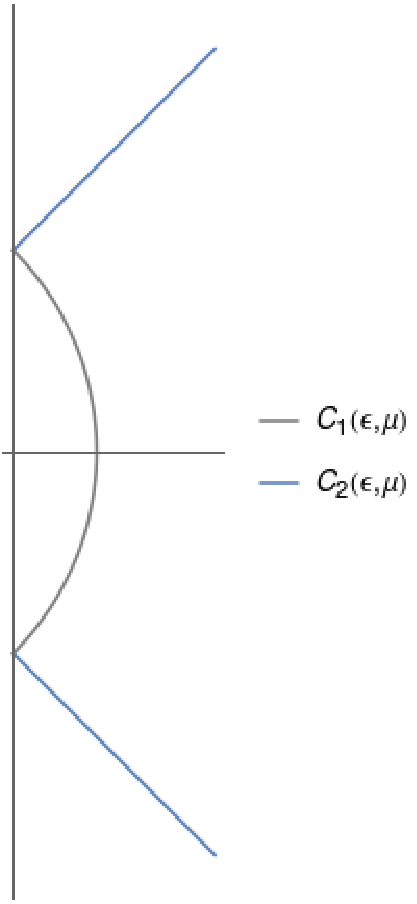
\includegraphics[width=0.6\columnwidth]{cbound.pdf}
\end{column}
\end{columns}

\end{frame}

\begin{frame}{An Expression for the Error}
From the previous we find
\[
E_{\alpha,\beta}(-A) = \frac{1}{2\alpha \pi i} \int_{C(\varepsilon,\mu) } \exp(\lambda^{\nicefrac{1}{\alpha}}) \lambda^{\nicefrac{1-\beta}{\alpha}} (\lambda I + A)^{-1} \,\textrm{d} \lambda, \quad \sigma(-A) \in G^-(\varepsilon,\mu),
\]
and together with
\[
R_m = E_{\alpha,\beta}(-A)\mathbf{v} - V_m E_{\alpha,\beta}(-H_m)\mathbf{e}_1, \quad m \geq 1,
\]
we write
\[
R_m = \frac{1}{2\alpha\pi i} \int_{C(\varepsilon,\mu)} \exp(\lambda^{\nicefrac{1}{\alpha}}) \lambda^{\nicefrac{1-\beta}{\alpha}} \delta_m(\lambda),\mathrm{d}\lambda,
\]
for 
\[
\begin{split}
\delta_m(\lambda) = &\; (\lambda I + A)^{-1}\mathbf{v} - V_m(\lambda I + H_m)^{-1}\mathbf{e}_1 \\
= &\; (\lambda I + A)^{-1}\mathbf{v} - V_m(\lambda I + H_m)^{-1}V_m^H \mathbf{v}.
\end{split} 
\]
\end{frame}

\begin{frame}{An Expression for the Error}
Observe now that
\[
\delta_m(\lambda) = (\lambda I + A)^{-1}\mathbf{v} - V_m(\lambda I + H_m)^{-1}V_m^H \mathbf{v} = \Delta_m \mathbf{v},
\]
\onslide<2->{By using the \alert{Arnoldi relation, since $\mathbf{v}_{m+1} \perp V_m$:}
\[
V_m^H (\lambda I + A) V_m = \lambda I + H_m,
\]
}
\onslide<3->{Therefore we have
\[
\Delta_m (\lambda I + A) V_m = 0.
\]
}
\onslide<4->{For an arbitrary $\mathbf{y} \in \mathbb{C}^m$ we have then
\[
(\lambda I + A)^{-1}\mathbf{v} - V_m(\lambda I + H_m)^{-1}V_m^H \mathbf{v} = \Delta_m (\mathbf{v} - (\lambda I + A)V_m \mathbf{y}) = \Delta_m p_m(A) \mathbf{v},
\]	
where $p_m(z)$ is a \alert{polynomial of degree $\leq m$} with $p_m(-\lambda) = 1$.
}
\end{frame}

\begin{frame}{An Expression for the Error}
We have therefore proved that 
\[
\|\delta_m(A)\| \leq \| (\lambda I + A)^{-1} - V_m (\lambda I + H_m)^{-1} V_m^H\| \|p_m(A)\mathbf{v}\|, \forall p_m \in \mathbb{P}_{\leq m}[z] \text{ with } p_m(-\lambda) = 1.
\]
By using \parencite[Lemma~2]{MR2486853} we also have the following expression
\[
\|\delta_m(\lambda)\| = \frac{\prod_{j=1}^{m} h_{j+1,j}}{|\det(\lambda I + H_m)|} \| (\lambda I + A)^{-1} \mathbf{v}_{m+1}\|.
\]
\onslide<2->{To obtain the first bound we call then
\[
D(\lambda) = \operatorname{dist}(\lambda,W(-A)) \quad \forall\,\lambda \in C(\varepsilon,\mu).
\]
}
\begin{block}<3->{Representation function}
Using (A1) and (A2) we can find a function $\nu(\varphi)$ such that
\[
\forall\,\lambda = |\lambda| \exp(\pm i \varphi) \in C(\varepsilon,\mu) \quad D(\lambda) \geq \nu(\varphi) |\lambda|, \quad \nu(\varphi) \geq \nu > 0.
\]
\end{block}

\end{frame}

\begin{frame}{A First Error Bound}
\begin{alertblock}{Theorem \parencite[Theorem~3.2]{MoretNovatiML}}
Let assumptions (A1) and (A2) hold, then for $m \geq 1$ and for every $M > 0$ we have
\[
\|R_m\| \leq \frac{\exp(M) \prod_{j=1}^{m} h_{j+1,j} }{\pi \nu^{m+1} M^{m\alpha+\beta-1}} \left( \frac{\mu}{\alpha} + \frac{\exp(-M(|\cos(\nicefrac{\mu}{\alpha})| + 1))}{m\alpha-1+\beta} \right).
\]
\end{alertblock}

\onslide<2->{\textbf{Proof.} We use $\|(\lambda I + A)^{-1}\| \leq D(\lambda)^{-1}$ and $W(H_m) \subseteq W(A)$ in the error expression $R_m$
\only<2>{\[
\begin{split}
\| R_m \| = & \left\| \frac{1}{2\alpha\pi i} \int_{C(\varepsilon,\mu)} \exp(\lambda^{\nicefrac{1}{\alpha}}) \lambda^{\nicefrac{1-\beta}{\alpha}} \delta_m(\lambda),\mathrm{d}\lambda \right\| \\
\leq & \frac{\prod_{j=1}^{m} h_{j+1,j} }{2\pi \alpha} \int_{C(\varepsilon,\mu)} \frac{\left| \exp(\lambda^{\nicefrac{1}{\alpha}}) \lambda^{\nicefrac{1-\beta}{\alpha}} \right| }{D(\lambda)^{m+1}}\,|\mathrm{d}\lambda|.
\end{split}
\]
}%
\only<3>{
\[
\| R_m \| \leq \frac{\prod_{j=1}^{m} h_{j+1,j} }{2\pi \alpha} (I_1 + I_2),
\]	
with
\[
I_1 = \int_{C_1(\varepsilon,\mu)} \frac{\left| \exp(\lambda^{\nicefrac{1}{\alpha}}) \lambda^{\nicefrac{1-\beta}{\alpha}} \right| }{D(\lambda)^{m+1}}\,|\mathrm{d}\lambda| \leq 2 \varepsilon^{\frac{1-\beta}{\alpha}-m} \int_{0}^{\mu} \frac{\exp(\varepsilon^{\nicefrac{1}{\alpha}} \cos(\nicefrac{\varphi}{\alpha}) )}{\nu(\varphi)^{m+1}}\,\mathrm{d}\varphi,
\]
}
\only<4>{\vspace{-0.3em}
	\[
	\| R_m \| \leq \frac{\prod_{j=1}^{m} h_{j+1,j} }{2\pi \alpha} \left( 2 \varepsilon^{\frac{1-\beta}{\alpha}-m} \int_{0}^{\mu} \frac{\exp(\varepsilon^{\nicefrac{1}{\alpha}} \cos(\nicefrac{\varphi}{\alpha}) )}{\nu(\varphi)^{m+1}}\,\mathrm{d}\varphi + I_2 \right),
	\]	
	with\vspace{-0.5em}
	\[
	\begin{split}
	I_2 = & \int_{C_2(\varepsilon,\mu)} \frac{\left| \exp(\lambda^{\nicefrac{1}{\alpha}}) \lambda^{\nicefrac{1-\beta}{\alpha}} \right| }{D(\lambda)^{m+1}}\,|\mathrm{d}\lambda| \leq \frac{2}{\nu^{m+1}} \int_{\varepsilon}^{+\infty} \frac{r^{\frac{1-\beta}{\alpha}} \exp( -r^{\frac{1}{\alpha}} | \cos(\nicefrac{\mu}{\alpha}) |)  }{r^{m+1}}\,\mathrm{d}r \\ = & \frac{2}{\nu^{m+1}} \int_{\varepsilon^{\nicefrac{1}{\alpha}}}^{+\infty}
	\frac{\exp(-s |\cos(\nicefrac{\mu}{\alpha})|)}{s^{m\alpha+\beta}}\,\mathrm{d}s \leq \frac{2 \alpha \exp(-\varepsilon^{\nicefrac{1}{\alpha}} |\cos(\nicefrac{\mu}{\alpha})| ) }{(m\alpha+\beta-1) \nu^{m+1} \varepsilon^{\frac{m\alpha+\beta-1}{\alpha}}}.
	\end{split}
	\]
}
\only<5->{
\[
	\| R_m \| \leq \frac{\prod_{j=1}^{m} h_{j+1,j} }{2\pi \alpha} \left( 2 \varepsilon^{\frac{1-\beta}{\alpha}-m} \int_{0}^{\mu} \frac{\exp(\varepsilon^{\nicefrac{1}{\alpha}} \cos(\nicefrac{\varphi}{\alpha}) )}{\nu(\varphi)^{m+1}}\,\mathrm{d}\varphi +
\frac{2 \alpha \exp(-\varepsilon^{\nicefrac{1}{\alpha}} |\cos(\nicefrac{\mu}{\alpha})| ) }{(m\alpha+\beta-1) \nu^{m+1} \varepsilon^{\frac{m\alpha+\beta-1}{\alpha}}}
\right)
\]	
The result follows then by setting $\varepsilon = M^\alpha$ and simplifying the expression. \hfill\qedsymbol
}
}

\only<6->{\vfill
\alert{\faExclamationTriangle}\; With the same proof another bound for the case of small $\alpha$ can be obtained.
}
\end{frame}

\begin{frame}{A First Error Bound: small $\alpha$s}

\begin{alertblock}{Theorem \parencite[Theorem~3.2]{MoretNovatiML}}
	Let assumptions (A1) and (A2) hold, then for $m \geq 1$ and for every $M > 0$ we have
	\[
	\|R_m\| \leq \frac{\exp(M) \prod_{j=1}^{m} h_{j+1,j} }{\pi \nu^{m+1} M^{m\alpha+\beta-1}} \left( \frac{\mu}{\alpha} + \frac{\exp(-M(|\cos(\nicefrac{\mu}{\alpha})| + 1))}{m\alpha-1+\beta} \right).
	\]
\end{alertblock}

\begin{alertblock}{Corollary \parencite[Corollary 3.3]{MoretNovatiML} }
Let assumptions (A1) and (A2) hold. Let $m \geq 1$ be such that $m \alpha + \beta > 0$, then for every $M>0$, we have
\[
\|R_m\| \leq \frac{\exp(M) \prod_{j=1}^{m} h_{j+1,j} }{4\nu^{m+1}M^{m\alpha}} \frac{4 M^{1-\beta}}{\pi} \left(\frac{\mu}{\alpha} + \frac{\exp(-M(1 + |\cos(\nicefrac{\mu}{\alpha})|))}{M |\cos(\nicefrac{\mu}{\alpha})| } \right).
\]
\end{alertblock}

\end{frame}


\begin{frame}{A First Error Bound: some observations}

\begin{itemize}
	\item<1->[\faCog] The ML function is entire for $\alpha > 0$ $\Rightarrow$ superlinear convergence for large enough $m$:
	\[
	M = m\alpha + \beta -1 \;\Rightarrow\; \|R_m\| \propto \left( \frac{\exp(1)}{M} \right)^M \nu^{-(m+1)} \prod_{j=1}^{m} h_{j+1,j}.
	\]
	\item<2->[\faCog] To better understand this, we use that for every monic polynomial of degree $m$ we find
	\[
	\prod_{j=1}^{m} h_{j+1,j} \leq \only<2>{\|q_m(A) v \|}\only<3->{2 \gamma^m},
	\]
	Therefore, if we take $q_m$ as the \alert{\textbf{monic Faber polynomial}} associated to a closed convex subset $\Omega \supset W(-A)$ we get the bound in terms of the \textbf{logarithmic capacity} $\gamma$ of $\Omega$.
	\item<3->[$\Rightarrow$] we have discovered:
	\[
	\|R_m\| \propto \left( \frac{\exp(1)}{m\alpha} \right)^{m\alpha} \left( \frac{\gamma}{\nu} \right)^m.
	\]
\end{itemize}

\end{frame}

\begin{frame}{Specialized bounds}
The bound can be refined under stricter hypotheses.

\begin{alertblock}<2->{Theorem \parencite[Theorem~3.5]{MoretNovatiML}}
Assume that $A$ is Hermitian with $\sigma(A) \subseteq [a,b] \subset [0,+\infty)$. Assume that $0 < \alpha < 1$, $\beta \geq \alpha$. Let $\mu \leq \nicefrac{\pi}{2}$, $\nicefrac{\alpha\pi}{2} < \mu < \alpha \pi$. Then for every index $m \geq 1$ and for every $M > 0$ we have
\[
\|R_m\| \leq \frac{4 M^{1-\beta}}{\pi} \left(\frac{\mu}{\alpha} + \frac{\exp(-M(1 + |\cos(\nicefrac{\mu}{\alpha})|))}{M |\cos(\nicefrac{\mu}{\alpha})| } \right) \exp(M) \Phi( u(M^\alpha \exp(i\mu) ) )^{-m}.
\]
for $\Phi(u) = u + \sqrt{u^2-1}$, $u(z) = \nicefrac{(|b+z|+|a+z|)}{b-a}$.
\end{alertblock}

\begin{exampleblock}<3->{Limiting relation}
If $\alpha \rightarrow 0$, $\beta = 1$, we have $E_{0,1}(-z) = (1+z)^{-1}$, $|z| < 1$. Then setting $\mu = \alpha \pi$ and letting $M=1$, we find\vspace{-0.5em}
\[
\|R_m\| \leq \frac{4 (\pi \exp(1)-\exp(-1)) }{\pi \Phi(u(1))^m}
\]
\end{exampleblock}

\end{frame}

\begin{frame}{The Shift-and-Invert Method~{\Large \parencite{MoretNovatiML}}}
We remain under the assumptions (A1) and (A2) and consider the matrix
\[
Z = (I + h A)^{-1}, \qquad h > 0,
\]
together with the space $\mathcal{K}_{m}(Z,\mathbf{v})$.

\onslide<2->{We can write the \alert{\textbf{analogous Arnoldi relation}} for $U_m = [\mathbf{u}_1,\ldots,\mathbf{u}_m]$ spanning $\mathcal{K}_{m}(Z,\mathbf{v})$:
\[
Z U_m = U_m S_m + s_{m+1,m} u_{m+1} \textbf{e}_m^T, \qquad S_m = U_m^H Z U_m.
\]
}

\onslide<3->{\vspace{-0.5em}The \textbf{approximation} is then given by
\[
\mathbf{y} = f(A)\mathbf{v} \approx \mathbf{y}_m = V_m f(B_m)\mathbf{e}_1 \text{ where } (I + h B_m)S_m = I.
\]}

\onslide<4>{\vspace{-0.5em}We can repeat the general error analysis using
\[
R_m = E_{\alpha,\beta}(-A)\mathbf{v} - U_m E_{\alpha,\beta}(-B_m)\mathbf{e}_1 = \frac{1}{2\pi \alpha i} \int_{C(\varepsilon,\mu)} \exp( \lambda^{\nicefrac{1}{\alpha}}) \lambda^{\nicefrac{(1-\beta)}{\alpha}} b_m(\lambda)\,\mathrm{d}\lambda, 
\]
for $b_m(\lambda) = (\lambda I + A)^{-1}\mathbf{v} - U_m (\lambda I + B_m)^{-1}\mathbf{e}_1$.
}
\end{frame}

\begin{frame}{Error bound~\parencite{MoretNovatiML}}

\begin{alertblock}{Theorem~\parencite[Theorem~4.3]{MoretNovatiML}}
For every matrix $A$ satisfying (A1) and (A2), assume $0 < \alpha < 1$ and $\beta \geq \alpha$. Then, there exists a function $g(h)$, continuous in any bounded interval $0 < h_1 \leq h \leq h_2$, such that for $m \geq 2$,\vspace{-0.5em}
\[
\|R_m\| \leq \frac{g(h)}{m-1}.
\]
\end{alertblock}

\begin{alertblock}<2->{Theorem~\parencite[Theorem~4.5]{MoretNovatiML}}
Assume that $A$ is Hermitian with $\sigma(A) \subseteq [a,+\infty)$, $a \geq 0$. Assume $0 < \alpha \leq \nicefrac{2}{3}$ and $\beta \geq \alpha$. Then, for every $m \geq 1$ we have\vspace{-0.5em}
\[
\|R_m\| \leq \frac{K_1 Q_m h^{\frac{\beta-1}{\alpha}}}{(1+\sqrt{2})^{m-1}} + \frac{K_2 h^{\nicefrac{\beta}{\alpha}}}{(m-1)^2} \exp\left( - \frac{ h^{-\nicefrac{1}{\alpha}}}{\sqrt{2}} \right),
\]
where 
$
Q_m = \max_{0 \leq |\varphi| \leq \nicefrac{3\alpha\pi}{4}} \exp\left( h^{-\nicefrac{1}{\alpha}} \cos \nicefrac{\varphi}{\alpha} \right) (1-\cos\varphi)^{\frac{m-1}{2}},
$
with $K_1$, $K_2$ constants.
\end{alertblock}

\end{frame}

\subsection{Conclusions}

\begin{frame}{ML function, what have we found?}

\begin{itemize}
	\item<1->[\faCog] The \emph{polynomial method} suffers both for \textbf{small $\alpha$ values} and for \textbf{large field of values}.
	\item<2->[\faCog] For the \emph{shift-and-invert} method the convergence doesn't deteriorate with the size of $W(A)$, its uniform with respect to the $h$ parameter. 
	\item<3->[\faWrench] To obtain a complete method one still has to find a way to repeatedly compute the matrix functions in\vspace{-0.5em}
	\[
	\mathbf{u}(t) = E_{\alpha,1}(-t^\alpha A) \mathbf{u}_0 + \int_{0}^{t} (t-s)^{\alpha-1} E_{\alpha,\alpha}(-A(t-s)^\alpha)\mathbf{g}(s)\,\textrm{d}s.
	\]
	\item<4->[\faBinoculars] \textbf{Research ideas:} finding better rational approximations/poles/expansions together with error analysis for the ML function.
\end{itemize}

\begin{exampleblock}<5->{Other extensions}
	A variant with \emph{restart} is discussed in~\parencite{MoretPopolizio}, the combination with other matrix-functions in~\parencite{MoretNovatiFDEfunction}.
\end{exampleblock}


\end{frame}




\appendix

\section*{Bibliography}
{\unnumbered
	\begin{frame}[allowframebreaks,noframenumbering]{Bibliography}
	\small
	\printbibliography
	
\end{frame}
}

\end{document}